\chapter{Complete set of rules for two and three part compositions}\label{appendix:complete-set-of-rule}
This appendix contains all the constraints for composing counterpoint for two or three voices. This appendix contains only the formalised equations, the corresponding explanations can be found in the corresponding sections of this thesis and that of T. Wafflard.

All the rules apply to three-voice compositions, but only the rules for two voices apply to two-voice compositions. Rules for three-part compositions are indicated by '3V' at the beginning of the rule.


Some of the rules are different depending on whether the composition is for two or three voices. In these cases, the mathematical relationship to be followed for the rule in question, depending on the situation, is clearly indicated.

\section*{Implicit General Rules of Counterpoint}


\begin{enumerate}[wide, label=\bfseries G\arabic*]
    \item \textit{Harmonic intervals are always calculated from the lower note.} \label{rule:hfromlower}

    Already handled by making the difference value absolute for the \textbf{H} variable. 

    \item \textit{The number of measures of the counterpoint must be the same as the number of measures of the \cfdot} \label{rule:sameNbMeasures}

    \begin{lstlisting}[caption=Definition of $N$ in the first species., label=lst:defcp, basicstyle=\ttfamily\small]
        (defvar *notes (list nil nil nil nil))
        ; ...
        ;; FIRST SPECIES ;;
        ; setting the first list of *notes with
        ;   integer *cf-len as size
        ;   set *extended-cp-domain as available notes
        (setf (first *notes)
            (gil::add-int-var-array-dom *sp* *cf-len *extended-cp-domain))
        \end{lstlisting}

    \item \textit{The counterpoint must have the same time signature and the same tempo as the \cfdot} \label{rule:sameTimeSignature}

    \begin{lstlisting}[caption=Definition of $N$ in the first species., label=lst:defcp, basicstyle=\ttfamily\small]
    (defvar *notes (list nil nil nil nil))
    ; ...
    ;; FIRST SPECIES ;;
    ; setting the first list of *notes with
    ;   integer *cf-len as size
    ;   set *extended-cp-domain as available notes
    (setf (first *notes)
        (gil::add-int-var-array-dom *sp* *cf-len *extended-cp-domain))
    \end{lstlisting}
    
    \item \textit{The counterpoint must be in the same key as the \cfdot}\label{rule:samekey}
    This rule is already handled by the creation of the set $\N$. The example of the actual rule given above will clarify the explanations. Let $k$ be the value of the key determined by the key signature, i.e. $60$ for $C$; and $t$ the tonic of the piece, i.e. $Cf[0]=65$. Then:

    \begin{equation*}
        \begin{gathered}
            \N_{key} = buildScale(k\ mod\ 12, "major") = \{0, 2, 4, 5, 7, 9, 11, 12, \dots, 127\}\\
            \N_{brw} = buildScale(t\ mod\ 12, "borrowed") = \{2, 4, 5, \textbf{10}, 14, \dots, 125\}\\
            \therefore \N_{all}=\{0, 2, 4, 5, 7, 9, \textbf{10}, 11, 12, \dots, 127\}
        \end{gathered}
    \end{equation*}

    To ensure that borrowed notes are used sparingly, they must be given a cost to use. Let $\mathit{Offkey}$ be the set of notes outside the key and $\mathit{Offkey}_{costs}$ the list of costs associated with each note. The cost for a note will be \textit{<no cost>} or $cost_{\mathit{Offkey}}$ (\dft{high cost}).

    \begin{equation}
        \begin{gathered}
            \mathit{Offkey} = [0, 1, 2, \dots, 127] \setminus \N_{key}\\
            % \forall c \in \mathit{Offkey}_{costs}, \forall p \in N \\
            % \forall \rho \in \mathcal{P}ositions\\
            \forp\\
            \mathit{Offkey}_{costs}[\rho] = \begin{cases}
                cost_{\mathit{Offkey}} & \text{if } N[\rho] \in \mathit{Offkey} \\
                0 & \text{otherwise}
            \end{cases}\\
            \text{moreover } \C = \C \cup \sum _{c \in \mathit{Offkey}_{costs}} c
        \end{gathered}
    \end{equation}

    \item \textit{The range of the counterpoint must be consistent with the instrument used.} \label{rule:instrurange}

    This rule is already handled by the creation of the set $\N^{\R} = \N \cap \R$. When $N$ is created its domain is set to $\N_{all}^{\R}$ as seen in the code sample \ref{lst:defcp}: \texttt{*extended-cp-domain} refers to the set $\N_{all}^{\R}$.

    \item \textit{Chromatic melodies are forbidden.}\label{rule:chromafb}

    \begin{equation}
        \begin{gathered}
            \forpmm\\
            (M_{brut}[\rho] = 1 \land M_{brut}[\rho+1] = 1) \iff \bot\\
            (M_{brut}[\rho] = -1 \land M_{brut}[\rho+1] = -1) \iff \bot\\
        \end{gathered}
    \end{equation}
    
    \item \textit{Melodic intervals should be small.}\label{rule:smallmelody}

    \begin{equation}\label{eq:mdeg_costs}
        \begin{gathered}
            \forpm\\
            Mdeg_{costs}[\rho] = \begin{cases}
                cost_{secondMdeg} & \text{if } M[\rho] \in \{0, 1, 2\}\\
                cost_{thirdMdeg} & \text{if } M[\rho] \in \{3, 4\}\\
                cost_{fourthMdeg} & \text{if } M[\rho] = 5\\
                cost_{tritoneMdeg} & \text{if } M[\rho] = 6\\
                cost_{fifthMdeg} & \text{if } M[\rho] = 7\\
                cost_{sixthMdeg} & \text{if } M[\rho] \in \{8, 9\}\\
                cost_{seventhMdeg} & \text{if } M[\rho] \in \{10, 11\}\\
                cost_{octaveMdeg} & \text{if } M[\rho] = 12\\
            \end{cases}\\
            \text{moreover } \C = \C \cup \sum _{c \in Mdeg_{costs}} c
        \end{gathered}
    \end{equation}

    \item\label{rule:last-chord-h-triad-appendix} \textit{3V - The last chord must be composed only of the notes of the harmonic triad.} 
\begin{equation} \begin{aligned}
    \forall s \in \{b, c\} \colon H(s)[0, m-1] \in Cons_{h\_triad}
\end{aligned} \end{equation}

\item \textit{3V - The last chord must have the same fundamental as the one of the scale used throughout the composition.}\label{rule:same-fundamental-appendix}
\begin{equation} \begin{aligned}
    N(a)[0, m-1] \mod 12 = N(cf)[0, 0] \mod 12
    \end{aligned} \end{equation}
\end{enumerate}


\section*{Constraints of the First Species}
\subsection*{Harmonic Constraints of the First Species}
\begin{enumerate}[wide, label=\bfseries 1.H\arabic*]
  \item\label{rule:allcons-appendix}{\textit{All harmonic intervals must be consonances.}} 
\begin{equation}
    \begin{gathered}
        \forall j \in [0, m)\quad 
        H[0, j] \in Cons
    \end{gathered}
\end{equation}

\item\label{rule:firstpcons}{\textit{The first harmonic interval must be a perfect consonance.}}
When dealing with two-part composition:
\begin{equation}
    \begin{gathered}
        H[0, 0] \in Cons_{p}
    \end{gathered}
\end{equation}
When dealing with three-part composition:
The rule doesn't exist.

\item\label{rule:lastpcons}{\textit{The last harmonic intervals must be a perfect consonance.}}
When dealing with two-part composition:
\begin{equation}
  \begin{gathered}
      H[0, m-1] \in Cons_{p}
  \end{gathered}
\end{equation}
When dealing with three-part composition:
The rule doesn't exist.

\item\label{rule:keytone}{\textit{The key tone is tuned according to the first note of the \cfdot}}

\begin{equation}
    \begin{gathered}
        \lnot \mathit{IsCfB}[0, 0] \implies H[0, 0] = 0\\
        \lnot \mathit{IsCfB}[0, m-1] \implies H[0, m-1] = 0
    \end{gathered}
\end{equation}

\item\label{rule:no-unison-appendix}{\textit{The voices cannot play the same note at the same time except in the first and last measure.}}

\begin{equation}
    \begin{gathered}
        \forall p_1, p_2 \in \{cf, cp_1, cp_2\}, \text{with} p_1 \neq p_2 \forall j \in \{0, 1, 2, 3\} \forall j \in [1, m-1) \quad
        N(p_1)[i, j] \neq N(p_2)[i, j]
    \end{gathered}
\end{equation}

\item \label{rule:prefer-imp-to-perf-appendix}{\textit{Imperfect consonances are preferred to perfect consonances.}}


\begin{equation}
    \begin{gathered}
        \forall j \in [0, m)\\
        Pcons_{costs}[j] = \begin{cases}
            cost_{Pcons} & \text{if } H[0, j] \in Cons_{p}\\
            0 & \text{otherwise}
        \end{cases}\\
        \text{moreover } \C = \C \cup \sum _{c \in Pcons_{costs}} c
    \end{gathered}
\end{equation}

\item{and \textbf{1.H8} \textit{The harmonic interval of the penultimate note must be a major sixth or a minor third depending on the \cfs pitch. When writing with three voices, the harmonic interval must be either a minor third, a perfect fifth, a major sixth or an octave.}}\label{rule:penult-interval-2v}
\addtocounter{enumi}{1} 
When dealing with two-part composition:
\begin{equation}
    \begin{gathered}
        % \lnot \mathit{IsCfB}[0, m-2] \implies H[0, m-2] = 9
        \rho := \max (positions(m)) - 1\\
        H[\rho] = \begin{cases}
            9 & \text{if } \mathit{IsCfB}[\rho]\\
            3 & \text{otherwise}
        \end{cases}\\
        \text{where } \rho \text{ represents the penultimate index of any counterpoint.}
    \end{gathered}
\end{equation}

When dealing with three-part composition:
\begin{equation}
    \begin{aligned}
        H[0, m-1] \in \{0, 3, 7, 9\}
    \end{aligned}
\end{equation}

\item  \textit{3V - One might use sixths or octaves.}
As discussed in \ref{rule:sixth-or-octaves}, there is no constraint to add for this rule.

\item \textit{3V - Tenths are prohibited in the last chord.}

\begin{equation} \begin{aligned}
&H_{brut}[0, m-1] > 12 \implies H[0, m-1] \notin \{3, 4\}
\end{aligned} \end{equation}

\item \textit{3V - Octaves should be preferred over unisons.}
As discussed in \ref{rule:unison-vs-octave}, there is no constraint to add for this rule.

\item \textit{3V - Last chord cannot include a minor third.}

\begin{equation} \begin{aligned}
H[0, m-1] \neq 3
\end{aligned} \end{equation}

\subsection*{Melodic Constraints of the First Species}
\end{enumerate}

\begin{enumerate}[wide, label=\bfseries 1.M\arabic*]
\item\label{rule:notritone}{\textit{Tritone melodic intervals are forbidden.} }

\begin{equation}
    \begin{gathered}
        \forpm\\
        M[\rho] = 6 \implies Mdeg_{costs}[\rho] = cost_{tritoneMdeg}\\
    \end{gathered}
\end{equation}

\item\label{rule:mlesixth}{\textit{Melodic intervals cannot exceed a minor sixth interval.}}

\begin{equation}
    \begin{gathered}
        \forj\quad
        M[0, j] \leq 8
    \end{gathered}
\end{equation}

\item \textit{3V - Steps are preferred to skips.}
This rule is a duplicate of rule \ref{rule:smallmelody}.

\item  \textit{3V - The notes of each part should be as diverse as possible.}
    \begin{equation} \begin{aligned}
    &\forall p \in \{cp_1, cp_2\}, \quad \forall j \in [0, m-1), \quad \forall k \in [j+1, \text{min} (j+3, m-1)] :\\ 
    &N(p)[0, j] = N(p)[0, j+k]\iff cost_{variety}[j+m*k]= 1
    \end{aligned} \end{equation}

    \item  \textit{Each part should stay in its voice range.}

This rule is already covered by the definition of the voice ranges, so no constraint is associated to it.

    \item  \textit{3V - Melodic intervals cannot be greater or equal to a sixth.}
    This rule is only a restatement of rule \ref{rule:mlesixth}, saying that melodic intervals cannot exceed a minor sixth interval.
\end{enumerate}
    
\subsection*{Motion Constraints of the First Species}
\begin{enumerate}[wide, label=\bfseries 1.P\arabic*]

\item\label{rule:nopconsbydm}{ \textit{Perfect consonances cannot be reached by direct motion.}}

When dealing with two-part composition:
\begin{equation}
    \begin{gathered}
        \forj\quad
        H[0, j+1] \in Cons_{p} \implies P[0, j] \neq 2
    \end{gathered}
\end{equation}

When dealing with three-part composition:
\begin{equation} \begin{aligned}
  &\forall j \in [0, m-2) :\\
  &P[0, j] = 2 \land H[0, j+1] \in Cons_{p} \\
  &\iff cost_{\text{{direct\_move\_to\_p\_cons}}}[j] = 8
\end{aligned} \end{equation}

\item\label{rule:codmotions} {\textit{Contrary motions are preferred to oblique motions which are preferred to direct motions.}}

\begin{multicols}{3}
    \begin{itemize}
        \item $cost_{con}$\\ \dft{no cost}
        \item $cost_{obl}$\\ \dft{low cost}
        \item $cost_{dir}$\\ \dft{medium cost}
    \end{itemize}
\end{multicols}

\begin{equation}
    \begin{gathered}
        \forj\\
        P_{costs}[j] = \begin{cases}
            cost_{con} & \text{if } P[0, j] = 0\\
            cost_{obl} & \text{if } P[0, j] = 1\\
            cost_{dir} & \text{if } P[0, j] = 2
        \end{cases}\\
        \text{moreover } \C = \C \cup \sum _{c \in P_{costs}} c
    \end{gathered}
\end{equation}

\item\label{rule:battuta}{ \textit{At the start of any measure, an octave cannot be reached by the lower voice going up and the upper voice going down more than a third skip.}}


\begin{equation}
    \begin{gathered}
        i := \max (\B), \forj\\
        H[0, j+1] = 0 \land P[i, j] = 0 \land \begin{cases}
            M_{brut}[i, j] < -4 \land \mathit{IsCfB}[i, j] \iff \bot\\
            M_{cf}[i, j] < -4 \land \lnot \mathit{IsCfB}[i, j] \iff \bot
        \end{cases}\\
        \text{where } i \text{ stands for the last beat index in a measure.}
    \end{gathered}
    \label{eq:battuta}
\end{equation}

\item \textit{3V - Successive perfect consonances should be avoided.}
\begin{equation} \begin{aligned}
    &\forall v_1, v_2 \in \{cf, cp_1, cp_2\}, \quad v_1 \neq v_2, \quad \forall j \in [0, m-2) \colon\\
    &(H(v_1,v_2)[0, j] \in Cons_) \land (H(v_1,v_2)[0, j+1] \in Cons_p)\\
    &\implies Cost_{succ\_p\_cons} = 2
    \end{aligned} \end{equation}

    \item  \textit{3V - Each part starts distant from the lowest stratum.}

    This is not a strict rule but an indication to make easier for the composer to have contrary motions. Since this is neither a requirement nor a preference, it can simply be added as a heuristic for the solver. This is discussed in section \ref{heuristics}, on heuristics.


    \item \textit{3V - It is prohibited that all parts move in the same direction.}

    To prevent this, we need only look at the motions between the parts and the lowest stratum. If one of their motions is contrary, then it is guaranteed that the three voices will not go in the same direction (because at least one is contrary). The same applies if one of the motions is oblique. The problem arises when all the movements are direct, because this would mean that the three voices are going in the same direction. So it was forbidden to have all motions direct at the same time.
    \begin{equation} \begin{aligned}
    &\forall j \in [0, m-2) \colon\\
    &\bigvee_{p \in \{cf, cp_1, cp_2\}}  M(p)[0, j] \neq 2
    \end{aligned} \end{equation}

    \item  \textit{3V - It is prohibited to use successive ascending sixths on a direct upwards motion.}
    Either the harmonic interval is not a sixth in any of both positions, or one of them is not moving up.

    \begin{equation}
        \begin{aligned}
            & \forall j \in [1, m-1), \quad \forall v_1, v_2 \in \{cf, cp_1, cp_2\} \text{ where } v_1 \neq v_2, \quad \text{sixth := } \{8,9\} \colon \\
            & (H(v_1, v_2)[0, j-1] \notin \text{sixth}) \lor (H(v_1, v_2)[0, j] \notin \text{sixth}) \\
            & \lor M(v_1)[0, j] > 0 \lor M(v_2)[0, j] > 0
        \end{aligned}
        \end{equation}

\end{enumerate}

\section*{Constraints of the Second Species}
\subsection*{Harmonic Constraints of the Second Species}
\begin{enumerate}[wide, label=\bfseries 2.H\arabic*]
\item\label{rule:consthesis}{ \textit{Thesis harmonies cannot be dissonant.}}

As explained above, there is no constraint to add because it would be a duplicate of rule \ref{rule:allcons}.

\item\label{rule:arsisdim}{\textit{Arsis harmonies cannot be dissonant except if there is a diminution.}}

\begin{equation}
    \begin{gathered}
        \forj\\
        IsDim[j] = \begin{cases}
            \top & \text{if } M^2[0, j] \in \{3, 4\} \land M^1[0, j] \in \{1, 2\} \land M^1[2, j] \in \{1, 2\}\\
            \bot & \text{otherwise}
        \end{cases}
    \end{gathered}
\end{equation}

\begin{equation}
    \begin{gathered}
        \forj \quad
        \lnot IsCons[2, j] \implies IsDim[j]
    \end{gathered}
\end{equation}

\item\label{rule:penult2nd} \label{rule:penultexception}{and \textbf{2.H4} \textit{In the penultimate measure the harmonic interval of perfect fifth must be used for the thesis note if possible. Otherwise, a sixth interval should be used instead.}}
\addtocounter{enumi}{1}

\begin{equation}
    \begin{gathered}
        H[0, m-2] \in \{7, 8, 9\}\\
        \therefore penulthesis_{cost} = \begin{cases}
            cost_{penulthesis} & \text{if } H[0, m-2] \neq 7\\
            0 & \text{otherwise}
        \end{cases}\\
        \text{moreover } \C = \C \cup penulthesis_{cost}
    \end{gathered}
\end{equation}

\item \textit{3V - Major thirds are now allowed in the last chord.}

No need to add a new constraint as this rule is already covered by rules \ref{rule:last-chord-not-perfect-anymore} and \ref{rule:harmonic-triad}.

\item \textit{3V - The half notes must be coherent with respect to the whole notes.}

No need to add a new constraint as this is not an actual rule.

\end{enumerate}

\subsection*{Melodic Constraints of the Second Species}
\begin{enumerate}[wide, label=\bfseries 2.M\arabic*]

\item\label{rule:octaveleap}{ \textit{If the two voices are getting so close that there is no contrary motion possible without crossing each other, then the melodic interval of the counterpoint can be an octave leap.}}

\begin{equation}
    \begin{gathered}
        \forj, \forall M_{cf}[j] \neq 0\\
        M[0, j] = 12 \implies (H_{abs}[0, j] \leq 4) \land (\mathit{IsCfB}[j] \iff M_{cf}[j]>0)
    \end{gathered}
\end{equation}

\item\label{rule:notsamecons}{ \textit{Two consecutive notes cannot be the same. When writing a three-part composition, the 4th-to-last, the 3rd-to-last and the 2nd-to-last may be the same.}}
When dealing with two-part composition:
\begin{equation}
    \begin{gathered}
        \forp \quad
        N[\rho] \neq N[\rho+1]
    \end{gathered}
\end{equation}

When dealing with three-part composition:
\begin{equation}
  \begin{aligned}
      &\forall j \in [1, m-1), \quad j \neq m-2:\\
      &((N[2, j-1] \neq N[0, j]) \land (N[0, j] \neq \land N[2, j])) \\
      &\land \\
      & ((N[2, m-3] \neq N[0, m-2]) \lor (N[0, m-2] \neq N[2, m-2]) )
  \end{aligned}
\end{equation}


\end{enumerate}
\subsection*{Motion Constraints of the Second Species}
\begin{enumerate}[wide, label=\bfseries 2.P\arabic*]

\item\label{rule:motion2nd}{\textit{If the melodic interval of the counterpoint between the thesis and the arsis is larger than a third, then the motion is perceived based on the arsis note.}}


\begin{equation}
    \begin{gathered}
        \forj \quad
        P_{real}[j] = \begin{cases}
            P[2, j] & \text{if } M[0, j] > 4\\
            P[0, j] & \text{otherwise}
        \end{cases}
    \end{gathered}
\end{equation}

\item\label{rule:battuta2}{ \textit{Rule \ref{rule:battuta} on the battuta octave is adapted such that it focuses on the motion from the note in arsis.}}
This constraint already had an adapted mathematical notation in the chapter of the first species. Note that this constraint would indeed use P[2] and not P$_{real}$.


\item \textit{3V - Successive fifths on the downbeat are only allowed when they are separated by a third on the upbeat.}    
    \begin{equation}
        \begin{aligned}
            & \forall p_1, p_2 \in \{cf, cp_1, cp_2\} \text{ where }  p_1 \neq p_2, \quad \forall j \in [0, m-2): \\
            &Cost_{succ\_p\_cons} = \,  
            \begin{cases}
                0 & \text{if } (H(p_1, p_2)[0, j] \notin Cons_p) \lor (H(p_1, p_2)[0, j+1] \notin Cons_p)\\
                0 & \text{if } (H(p_1, p_2)[0, j] = 5 ) \land (H(p_1, p_2)[0, j+1] = 5) \\
                & \quad \quad \quad \quad \quad \quad\land (H(p_1, p_2)[2, j] = 3) \lor (H(p_1, p_2)[2, j] = 4)\\
                2 & \text{otherwise } \\
            \end{cases}\\
        \end{aligned}
    \end{equation}

\end{enumerate}
%%%%%%%%%%%%%

\section*{Constraints of the Third Species}
\subsection*{Harmonic Constraints of the Third Species}
\begin{enumerate}[wide, label=\bfseries 3.H\arabic*]
  \item\label{rule:fivequarters}{ \textit{If five notes follow each other by joint degrees in the same direction, then the harmonic interval of the third note must be consonant.}}

\begin{equation}
    \begin{gathered}
        \forj\\
        % \{M[0, j]\land M[1, j]\land M[2, j]\land M[3, j]\} \leq 2\ \land\\
        % \left(
        %     \{M_{brut}[0, j]\land M_{brut}[1, j]\land M_{brut}[2, j]\land M_{brut}[3, j]\} > 0\ \lor \right. \\
        %     \left.
        %     \{M_{brut}[0, j]\land M_{brut}[1, j]\land M_{brut}[2, j]\land M_{brut}[3, j]\} < 0\
        % \right)\\
        % \implies IsCons[2, j]
        \left(
            \bigwedge_{i=0}^{3} M[i, j] \leq 2
        \right)
        \land
        \left(
            \bigwedge_{i=0}^{3} M_{brut}[i, j] > 0
            \lor
            \bigwedge_{i=0}^{3} M_{brut}[i, j] < 0
        \right)\\
        \implies IsCons[2, j]
    \end{gathered}
\end{equation}


\item\label{rule:thirddiss} {\textit{If the third harmonic interval of a measure is dissonant then the second and the fourth interval must be consonant and the third note must be a diminution.}}


\begin{equation}
    \begin{gathered}
        \forj\\
        IsCons[2, j] \lor \left( IsCons[1, j] \land IsCons[3, j] \land IsDim[j]\right)\\
        \text{where } IsDim[j]=\top \text{ when the \nth{3} note of the measure } j \text{ is a diminution.}
    \end{gathered}
\end{equation}

\item\label{rule:cambiata} {\textit{It is best to avoid the second and third harmonies of a measure to be consonant with a one-degree melodic interval between them.}}


\begin{equation}
    \begin{gathered}
        \forj\\
        Cambiata_{costs}[j] = \begin{cases}
            cost_{Cambiata} & \text{if } IsCons[1, j] \land IsCons[2, j] \land M[1, j] \leq 2\\
            0 & \text{otherwise}
        \end{cases}
    \end{gathered}
\end{equation}

\item\label{rule:penult3sp} {\textit{In the penultimate measure, if the \cfs is in the upper part, then the harmonic interval of the first note should be a minor third.}}

\begin{equation}
    \begin{gathered}
        \lnot \mathit{IsCfB}[m-2] \implies H[0, m-2] = 3
    \end{gathered}
\end{equation}

\item \textit{3V - The quarter notes must be coherent with respect to the whole notes.}
There is no constraint to add for this rule, which isn't really a rule.

\item \textit{3V - If the harmonic triad could not be used on the downbeat, it should be used on the second or third beat.}    
    \begin{equation} \begin{aligned}
            &\forall j \in [0, m-1) \colon \\
            &(H[1, j] \notin Cons_{h\_triad}) \land  (H[2, j] \notin Cons_{h\_triad})\\
            &\iff cost_{harmonic-triad-3rd-species}[j] = 1       
    \end{aligned} \end{equation}
\end{enumerate}


\subsection*{Melodic Constraints of the Third Species}
\begin{enumerate}[wide, label=\bfseries 3.M\arabic*]
  \item\label{rule:twobeats} {\textit{Each note and its two beats further peer are preferred to be different.}}


\begin{equation}
    \begin{gathered}
        \forpmm \\
        MtwoSame_{costs}[i, j] = \begin{cases}
            cost_{MtwobSame} & \text{if } M^2[\rho] = 0\\
            0 & \text{otherwise}
        \end{cases}
    \end{gathered}
\end{equation}
\end{enumerate}
\subsection*{Motion Constraints of the Third Species}
\begin{enumerate}[wide, label=\bfseries 3.P\arabic*]
  \item\label{rule:motion3rd} {\textit{The motion is perceived based on the fourth note.}}

This implies that the costs of the motions and the first species constraints on the motions are deducted from $P[3]$.
\end{enumerate}
%%%%%%%%%%%%%%%%%%%%%


\section*{Constraints of the Fourth Species}

\subsection*{Harmonic Constraints of the Fourth Species}
\begin{enumerate}[wide, label=\bfseries 4.H\arabic*]
  \item\label{rule:arsiscons} {\textit{Arsis harmonies must be consonant.}}

\begin{equation}
    \begin{gathered}
        \forall j \in [0, m-1) \quad
        H[2, j] \in Cons
    \end{gathered}
    \label{eq:arsiscons}
\end{equation}

\item\label{rule:noseventh} {\textit{If the \cfs is in the upper part, then no harmonic seventh interval can occur.}}

\begin{equation}
    \begin{gathered}
        \forall j \in [1, m-1) \quad
        \lnot \mathit{IsCfB}[j] \implies H[0, j] \notin \{10, 11\}
    \end{gathered}
\end{equation}

\item\label{rule:lowpenult4th} \label{rule:uppenult4th} {and \textbf{4.H4} \textit{In the penultimate measure, the harmonic interval of the thesis note must be a major sixth or a minor third depending on the \cfs pitch.}}

\begin{equation}
    \begin{gathered}
        H[0, m-2] = \begin{cases}
            9 & \text{if } \mathit{IsCfB}[m-2]\\
            3 & \text{otherwise}
        \end{cases}
    \end{gathered}
\end{equation}

\item \textit{3V - Imperfect consonances are preferred over fifth intervals, which in turn are preferred over octaves.}   

    This rule is already covered by rule \ref{rule:prefer-imp-to-perf-appendix} and by the default costs of the search.
\end{enumerate}
\subsection*{Melodic Constraints of the Fourth Species}
\begin{enumerate}[wide, label=\bfseries 4.M\arabic*]
  \item\label{rule:fullsyncopations} {\textit{Arsis half notes should be the same as their next halves in thesis.}}


\begin{equation}
    \begin{gathered}
        \forall j \in [0, m-1) \quad
        NoSync_{costs} = \begin{cases}
            cost_{NoSync} & \text{if } M[2, j] \neq 0\\
            0 & \text{otherwise}
        \end{cases}
    \end{gathered}
\end{equation}

\item\label{rule:m2same} {\textit{Each arsis note and its two measures further peer are preferred to be different.}}


\begin{equation}
    \begin{gathered}
        \forall j \in [0, m-1)\\
        MtwomSame_{costs} = \begin{cases}
            cost_{MtwomSame} & \text{if } N[2, j] = N[2, j+2]\\
            0 & \text{otherwise}
        \end{cases}
    \end{gathered}
\end{equation}

\end{enumerate}


\subsection*{Motion Constraints of the Fourth Species}
\begin{enumerate}[wide, label=\bfseries 4.P\arabic*]
  \item\label{rule:dissolved} {\textit{Dissonant harmonies must be followed by the next lower consonant harmony.}}

\begin{equation}
    \begin{gathered}
        \forall j \in [1, m-1) \quad
        \lnot IsCons[0, j] \implies M_{brut}[0, j] \in \{-1, -2\}
    \end{gathered}
\end{equation}

\item\label{rule:nosecond} {\textit{If the \cfs is in the lower part then no second harmony can be preceded by a unison/octave harmony.}}

\begin{equation}
    \begin{gathered}
        \forall j \in [1, m-1)\\
        \mathit{IsCfB}[j+1] \implies H[2, j] \neq 0 \land H[0, j+1] \notin \{1, 2\}
    \end{gathered}
\end{equation}

\item \textit{3V - Successive fifths are allowed when using ligatures.}    

    \begin{equation} \begin{aligned}
        &\forall v_1, v_2 \in \{cf, cp_1, cp_2\}, \quad \text{with } v_1 \neq v_2, \quad \forall j \in [0, m-2) \colon\\
        &Cost_{succ\_p\_cons} = \,  
        \begin{cases}
            0 & \text{if } (H(p_1, p_2)[0, j] \notin Cons_p) \lor (H(p_1, p_2)[0, j+1] \notin Cons_p)\\
            0 & \text{if } (H(p_1, p_2)[0, j] = 5 ) \land (H(p_1, p_2)[0, j+1] = 5) \\
            2 & \text{otherwise } \\
        \end{cases}\\
    \end{aligned} \end{equation}


    \item \textit{3V - Resolving to a fifth is preferred over resolving to an octave.}    
    
    This is already covered by the rule \ref{rule:prefer-fifths-over-octaves} (prefer fifths over octaves), since preferring fifths over octaves in \textit{all} cases implies preferring to resolve to a fifth rather than to an octave.

    \item \textit{3V - Stationary movement in the bass implies dissonance in the fourth species part.}

    \begin{equation}
        \begin{aligned}
        &\forall j \in [0, m-1):\\
        &M(a)[0, j] \neq 0 \iff H[2, j] \in Cons\\
        &M(a)[0, j] = 0 \iff H[2, j] \in Dis
        \end{aligned}
    \end{equation}        


    \item \textit{3V - A note provoking a hidden fifth gets replaced by a rest.}
    \begin{equation}
        \begin{aligned}
            &\forall j \in [1, m-1):\\
            &H[0, j] = 7 \land P[0,j] = 2 \iff N(0, j-1) = \emptyset  
        \end{aligned}
    \end{equation}

\end{enumerate}
%%%%%%%%%%%%%%
\section*{Constraints of the Fifth Species}
The fifth type has a very specific way of working, which cannot be summarised as easily as the other types, as it requires some additional concepts. We here provide the main concepts but for a fully understand of this species' formalisaiton, please refer to Chapter 7 of T. Wafflard's thesis.

First of all, here is the formal definition of S:
\begin{equation}
    \begin{gathered}
        \forp\\
        S[\rho] = \begin{cases}
            0 & \text{if } N[\rho] \text{ is not constrained by any species}\\
            1 & \text{if } N[\rho] \text{ is constrained by the first species}\\
            2 & \text{if } N[\rho] \text{ is constrained by the second species}\\
            3 & \text{if } N[\rho] \text{ is constrained by the third species}\\
            4 & \text{if } N[\rho] \text{ is constrained by the fourth species}\\
        \end{cases}\\
    \end{gathered}
\end{equation}

And the formal definition of IsS$_\text{x}$:
\begin{equation}
    \begin{gathered}
        \forall x \in \{0, 1, 2, 3, 4\}, \forp\\
        IsS_{x}[\rho] = \begin{cases}
            \top & \text{if } S[\rho] = x\\
            \bot & \text{otherwise}
        \end{cases}\\
    \end{gathered}
\end{equation}


\begin{enumerate}[wide, label=\bfseries 5.R\arabic*]
    \item  \label{rhythm:taexist} \textit{There must always be a note in thesis and in arsis, except the very first thesis and the very last arsis.}
       \begin{equation}
        \begin{gathered}
            \forall j \in [0, m)\\
            \lnot IsS_{0}[0, j]\quad \text{ where } j \neq 0\\
            \lnot IsS_{0}[2, j]\quad \text{ where } j \neq m-1
        \end{gathered}
    \end{equation}

    \item \label{rhythm:no4in2and4} \textit{The \species{4} can only exist in first and third beat.}
    
    \begin{equation}
        \begin{gathered}
            \forall i \in \{1, 3\}, \forall j \in [0, m)\quad
            \lnot IsS_{4}[i, j]
        \end{gathered}
    \end{equation}

    \item \label{rhythm:404} \textit{A \species{4} in the third beat necessarily implies a \species{4} in the first beat of the following measure and vice versa. The fourth beat should then have no note.}
    
    \begin{equation}
        \begin{gathered}
            \forall j \in [0, m-1)\\
            IsS_{4}[2, j] \iff IsS_{4}[0, j+1]\\
            IsS_{4}[2, j] \implies IsS_{0}[3, j]
        \end{gathered}
    \end{equation}

    \item \label{rhythm:no0after3} \textit{A \species{3} cannot be followed by no note.}
    
    \begin{equation}
        \begin{gathered}
            \forpm\quad
            IsS_{3}[\rho] \implies \lnot IsS_{0}[\rho+1]
        \end{gathered}
    \end{equation}

    \item \label{rhythm:not12} \textit{Only \species{3} and \species{4} are used.}

    \begin{equation}
        \begin{gathered}
            \forp\quad
            \lnot IsS_{1}[\rho] \land \lnot IsS_{2}[\rho]
        \end{gathered}
    \end{equation}

    \item \label{rhythm:syncinfirstpenult} \textit{The first and penultimate measures are linked to the \species{4}.}
        
    \begin{equation}
        \begin{gathered}
            IsS_{0}[0, 0] \land IsS_{0}[1, 0] \land IsS_{4}[2, 0]\\
            IsS_{4}[0, m-2] \land IsS_{0}[1, m-2] \land IsS_{4}[2, m-2]
        \end{gathered}
    \end{equation}
\end{enumerate}

\subsection*{Generalisation of the Species implications}

\begin{equation}
    \begin{gathered}
        \forall x \in \{3, 4\}, \forall cst_{x} \in Constraints(x), \forall V \in Variables(cst_{x})\\
        \left(\bigwedge_{\forall v \in V} IsS_{x}[v_{pos}]\right) \implies cst_{x}(V)\\
        \text{where }Constraints(x) \text{ is the set of constraints of the species }x,\\
        \text{and }Variables(cst_{x}) \text{ is the set of set of variables concerned by the constraint }cst_{x},\\
        \text{and }v_{pos} \text{ is the position of the } v \text{ related note in the array }N.\\
    \end{gathered}
\end{equation}

\subsection*{Avoiding Multiple Same Final Solutions}
\begin{equation}
    \begin{gathered}
        \forpm\quad
        IsS_{0}[\rho] \implies (N[\rho] = N[\rho + 1])
    \end{gathered}
\end{equation}

\subsection*{Formalization of Inter-species Rules into Constraints}
\begin{equation} \label{eq:syncopationvariation}
    \begin{gathered}
        \forall j \in [1, m-1)\\
        \lnot IsCons[0, j] \land IsS_{4}[0, j] \implies M^{2}_{brut}[0, j] \in \{-1, -2\} \land IsCons[2, j]
    \end{gathered}
\end{equation}

\subsection*{Parsing of the Species Array in Rhythm}
The fifth species is unique as it is the only one that might have a different rythm in each beat. To handle this, a parsing is applied after a solution is found to determine the rhythm of the counterpoint.

This parsing is shown in Figure \ref{fig:rhythmdiagram}. The letters correspond to the following: N are the notes the final counterpoint (the one that is returned), Cp are the notes computed by the solver (the array used by the solver), R is the rhythm and S is the S array.

\begin{figure}[]
    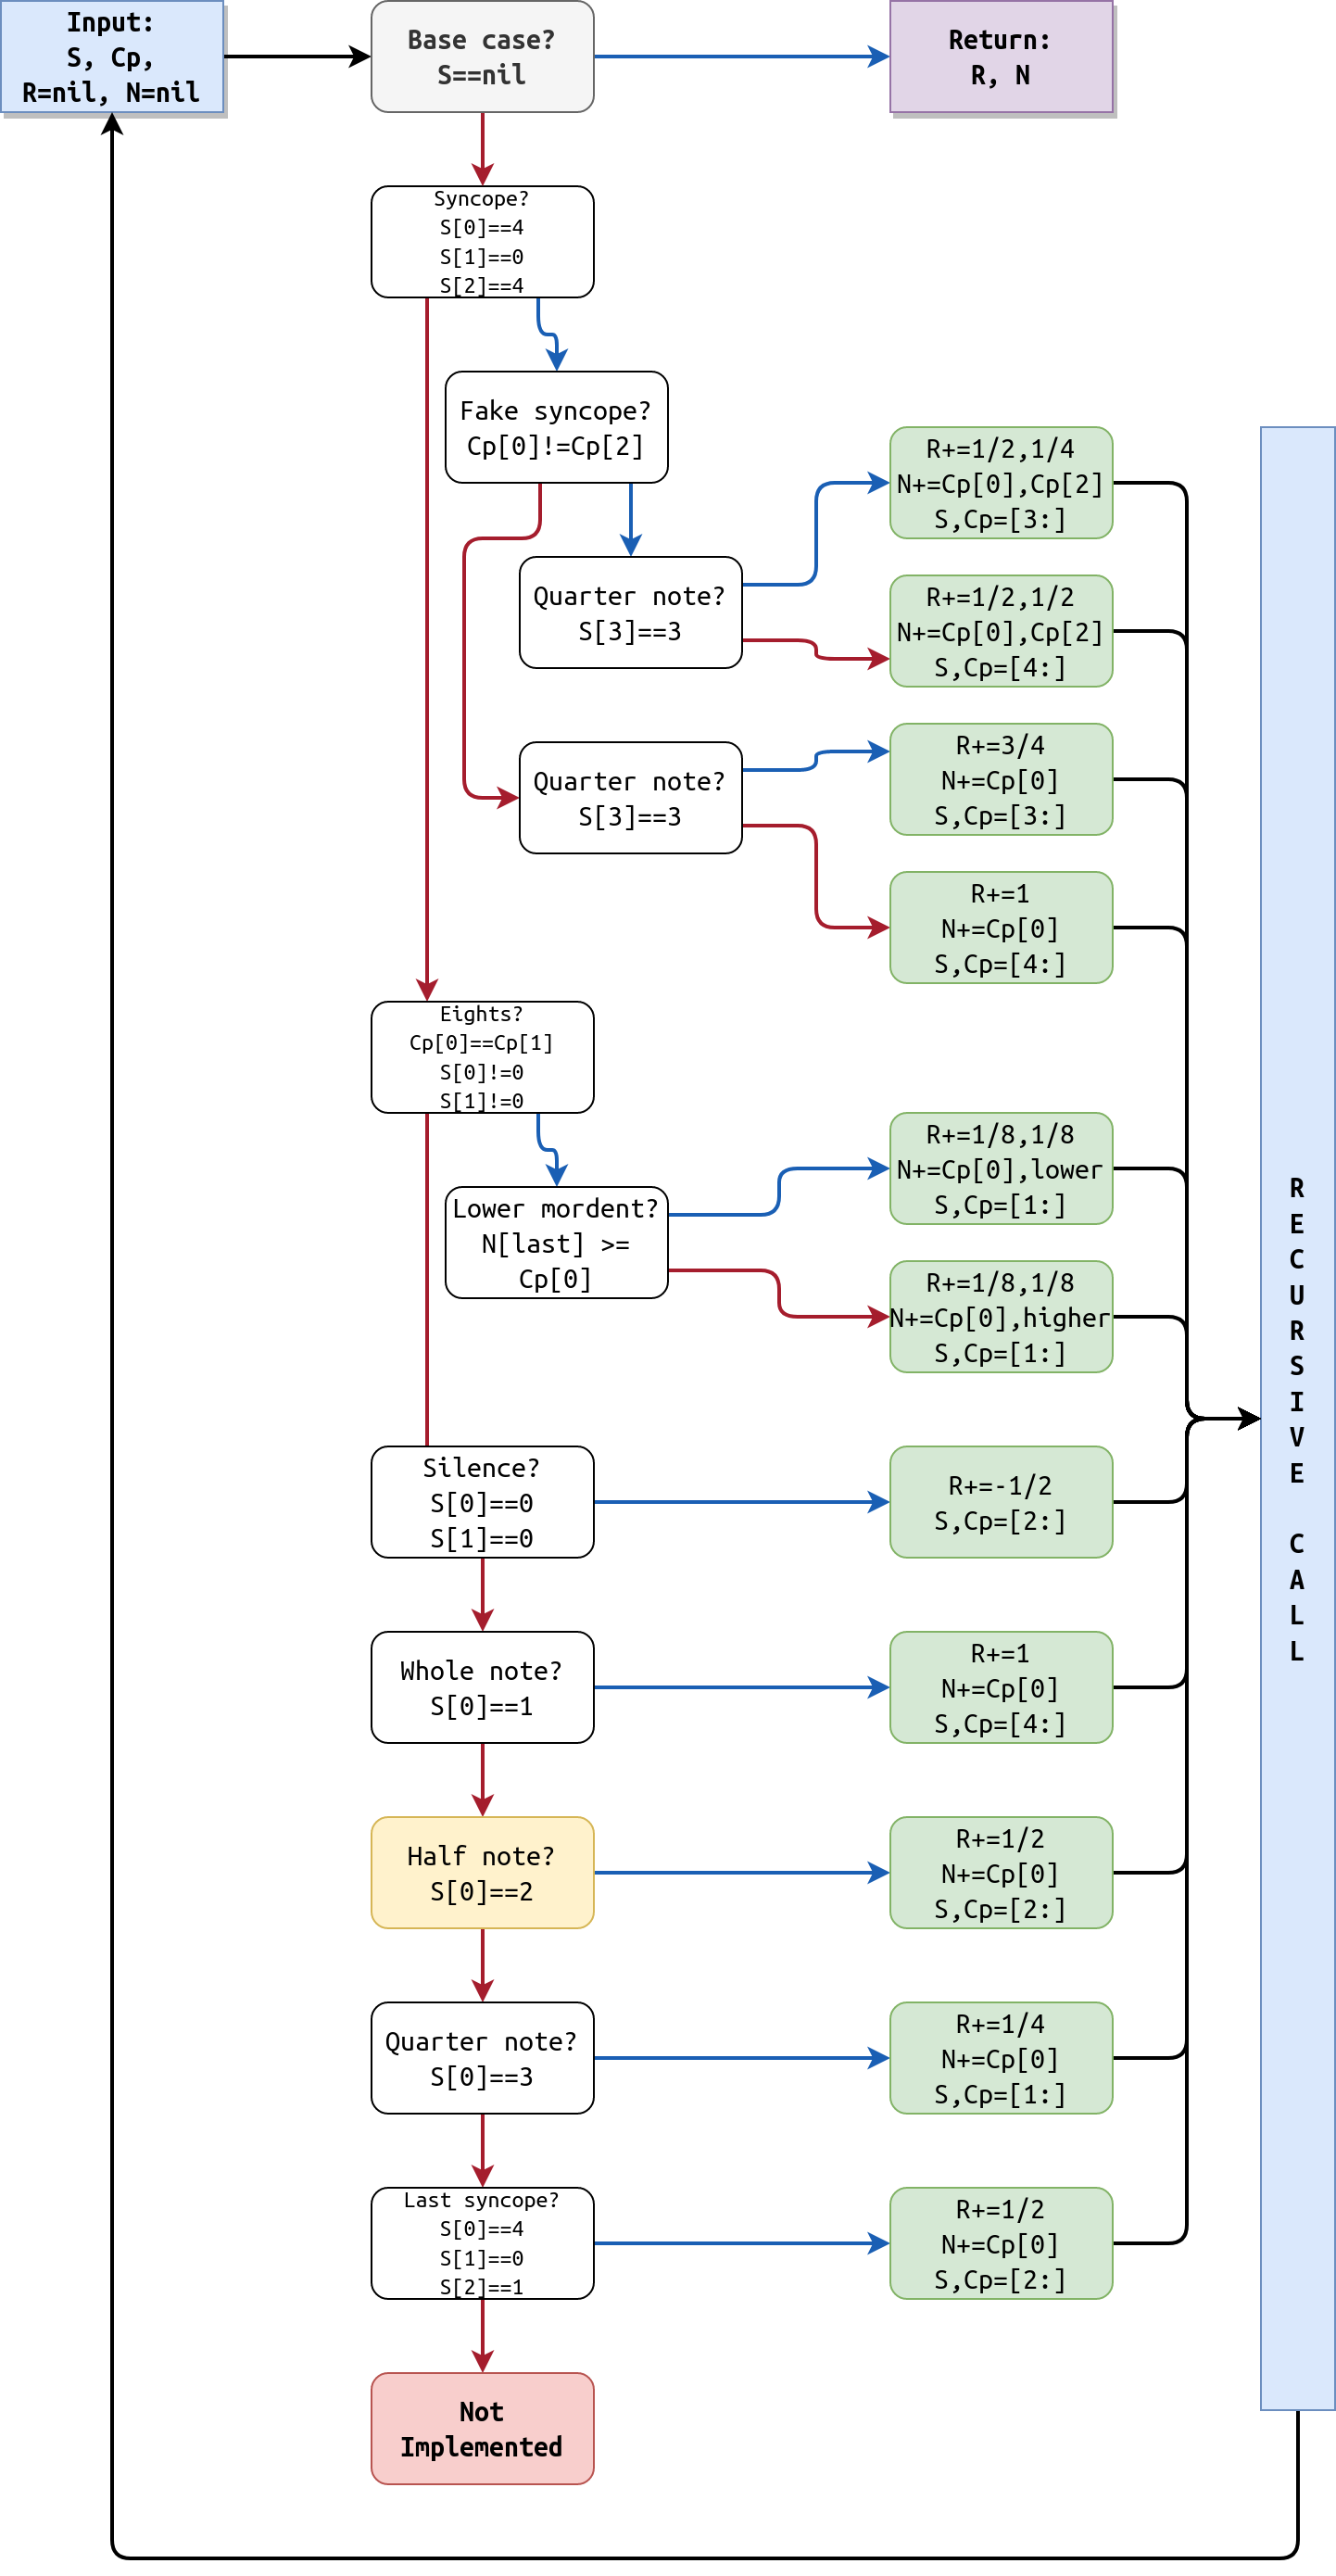
\includegraphics[scale=0.23, center]{Images/build_rhythmic_pattern.png}
    \caption{Rhythm species parser algorithm diagram, \species{5}. A \textcolor{red}{red arrow} means the test failed while a \textcolor{blue}{blue one} means it passed.}
    \label{fig:rhythmdiagram}
\end{figure}